% !TEX program = xelatex

% ==== Part1: 引入latex需要的package,支持不同的需求,如中文、图片 ====
\documentclass{article}
\usepackage[UTF8]{ctex} % 中文latex支持
\usepackage{graphicx} % 引入图片时需要的包
\usepackage{float}    % 插入图片的时候支持`H`这个位置选项
\usepackage{subcaption} % 插入多张图片到一个figure域中
\usepackage{hyperref}   % 插入超链接、TOC支持链接
% ==== 对引入的package配置 ====
\graphicspath{{images/}} % 配置graphicx这个包:指定图片存储的地方
\hypersetup{ % 设置超链接和url的显示样式
    colorlinks=true,
    linkcolor=blue,
    filecolor=magenta,      
    urlcolor=cyan,
    pdftitle={Overleaf Example},
    pdfpagemode=FullScreen,
    }
\urlstyle{same}

% ==== Part2: latex文档格式配置 ====
\newif\ifchinese % 定义一个条件变量: ifchinese, 作为控制条件编译的开关
\chinesetrue % 条件编译的控制开关,注释掉此部分内容,则对应部分不会被现实

% ==== Part3: latex文档标题部分 ====
\title{LaTex文档模版}
\author{付杰\thanks{谢谢overleaf提供的LaTex教程}}
\date{\today}


% ==== Part4: latex文档正文部分 ====
\begin{document}
\maketitle
\newpage

\tableofcontents % 插入目录
\newpage

\begin{abstract} % 摘要
  这部分是摘要的内容,基本上论文都是需要摘要的 这个文档是我在学习LaTex的时候做练习使用的文档,本文的组织架构如下,第1部分首先确定了本文档的结构,分别是“引入的包"、“对包的配置”、“LaTex文档的配置”、“LaTex的正文部分”。第2部分介绍了LaTex的技巧、如“条件编译”,“插入图片”、“插入公式”等
  \par\textbf{关键字:}LaTex结构、LaTex语法
\end{abstract}
\newpage



\section{条件编译:根据配置的信息,选择编译某一部分的内容}

\ifchinese
这部分是条件编译的内容,必须在\textbf{chinesetrue}判定为真的时候,才会被输出
\fi


\section{引入参考文献}
这部分内容饮用了参考文献\cite{ar1}


\section{插入图片}
\subsection{插入单张图片}
我们可以使用\textbf{includegraphics}来插入一个图片,例如图\ref{fig:mesh1} % ref可以引用一个label对应的图、表


\begin{figure}[ht] % h: approximate here, t: top of page
% \begin{figure}[H] % H: 准确的插入图片于here, 需要包float
    \centering % 图片居中
    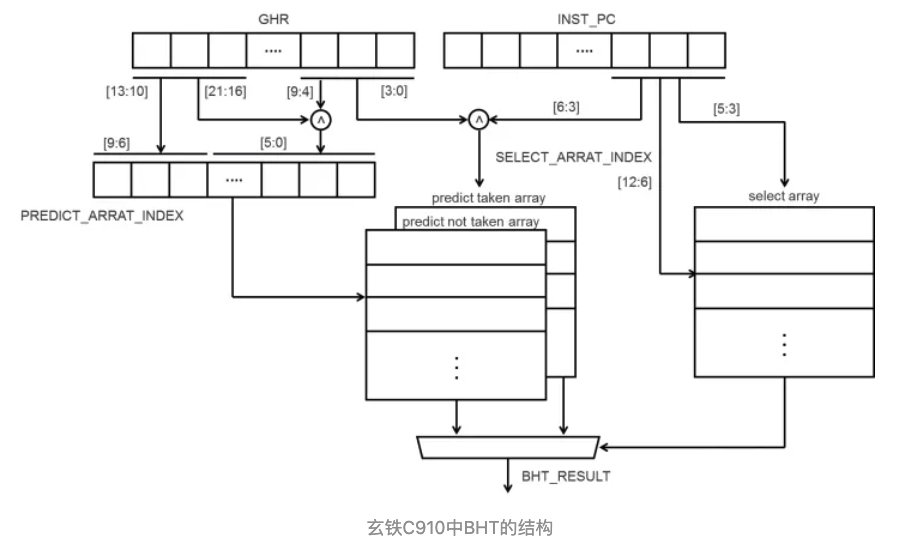
\includegraphics[width=0.75\textwidth]{C910BHT.jpg} % 插入图片
    \caption{A nice plot.} % 图片的注释
    \label{fig:mesh1} % 图片的lable,在文档中可以通过label引用图片
\end{figure}

这个图片的例子在第\pageref{fig:mesh1}页 % pageref可以指明label所在的页数

\subsection{插入两张图片}
  插入两个图片必须使用包\textbf{subcaption},在第\pageref{fig:subim1}页的这个例子中,我们插入了两个子图片,图\ref{fig:subim2}是第二个子图。

  \begin{figure}[ht]
    \begin{subfigure}{0.5\textwidth}
      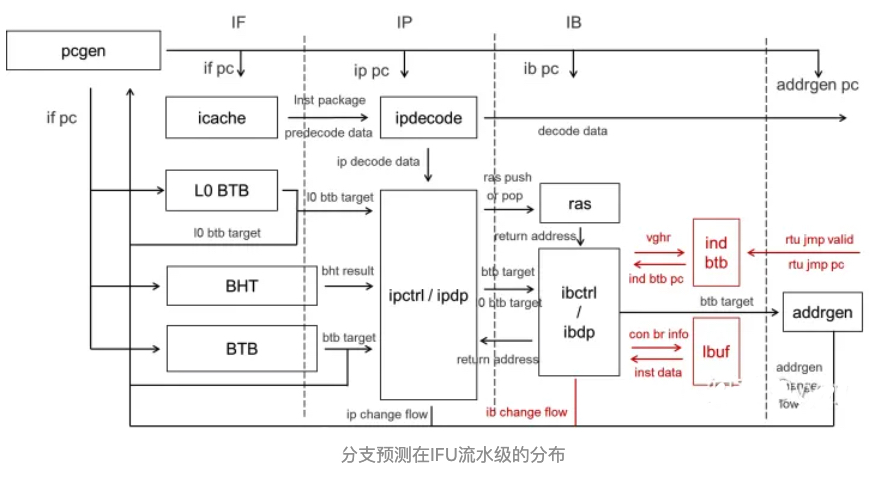
\includegraphics[width=0.9\linewidth, height=6cm]{bp01.jpg} 
      \caption{Caption1}
      \label{fig:subim1}
    \end{subfigure}
    \begin{subfigure}{0.5\textwidth}
      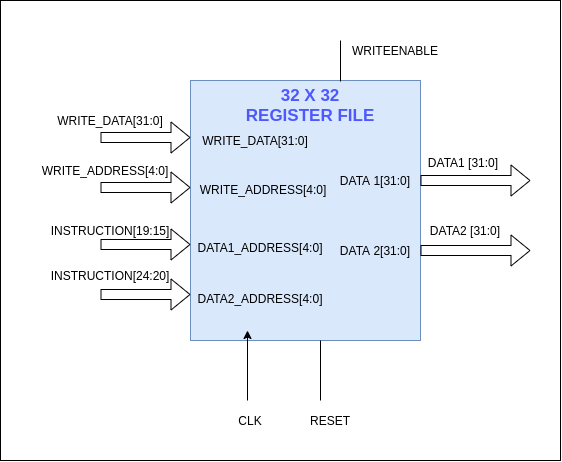
\includegraphics[width=0.9\linewidth, height=6cm]{reg_file.png}
      \caption{Caption 2}
      \label{fig:subim2}
    \end{subfigure}

    \caption{Caption for this figure with two images}
    \label{fig:image2}
  \end{figure}

\section{插入数学公式}
\begin{itemize}
  \item 插入行内公式:$e=m^2$
  \item 插入整行的公式: 
        \[ 
           f'(x)=\frac{dx}{dy}
        \]
  \item 插入带标号的公式
        \begin{equation}
         f=ma 
          \label{eq:1}
        \end{equation} 
\end{itemize}

  带标号的公式可以被我们引入,公式\ref{eq:1}表明了加速度和力大小的关系

\section{插入表格}
  表格\ref{table:data}是带注释和标号的表格
  \begin{table}[H]
  \centering
    \begin{tabular}{||c c c c||}  % 插入竖线
     \hline % 插入横线
     Col1 & Col2 & Col2 & Col3 \\ [0.5ex] 
     \hline\hline
     1 & 6 & 87837 & 787 \\ 
     2 & 7 & 78 & 5415 \\
     3 & 545 & 778 & 7507 \\
     4 & 545 & 18744 & 7560 \\
     5 & 88 & 788 & 6344 \\ [1ex] 
     \hline
    \end{tabular} % 表格主体
  \caption{带标号和注释的表格.}
  \label{table:data}
  \end{table}
  

\section{超链接}
本文的参考文献有: 

\begin{enumerate}
  \item \href{https://www.overleaf.com/learn/latex/Learn_LaTeX_in_30_minutes}{Overleaf的LaTex 30分钟教程}
  \item \href{https://www.overleaf.com/learn/latex/Hyperlinks#Introduction}{LaTex使用超链接hyperref}
  \item \href{https://www.overleaf.com/learn/latex/Positioning_images_and_tables}{LaTex插入图片}, 
\end{enumerate}


\newpage
\bibliography{ref} % 参考文献源,存储所有的参考文献
\bibliographystyle{IEEEtran} % latex饮用参考文献时的格式

\end{document}

